\documentclass{article}

\usepackage{fullpage}
\usepackage{multicol}
\usepackage{amsmath}
\usepackage{amssymb}
\usepackage{mathtools}
\usepackage{bm}
\usepackage{tikz}
\usetikzlibrary{shapes.geometric, positioning}
\usepackage{float}

% Macros
\newcommand{\R}{\mathbb{R}}
\newcommand{\N}{\mathbb{N}}
\newcommand{\Q}{\mathbb{Q}}
\renewcommand{\vec}[1]{\underline{\textbf{#1}}}
\newcommand{\veci}{\bm{\hat{\imath}}}
\newcommand{\vecj}{\bm{\hat{\jmath}}}
\newcommand{\veck}{\bm{\hat{k}}}
\newcommand{\e}{\varepsilon}
\newcommand{\de}{\delta}
\newcommand{\kd}{\delta_{i, j}}
\newcommand{\at}{\e_{i, j, k}}
\newcommand{\nab}{\underline{\nabla}}
\newcommand{\grad}{{\nab}\, f}
\newcommand{\pd}[2]{\frac{\partial #1}{\partial #2}}
\renewcommand{\div}{\nab \cdot}
\newcommand{\curl}{\nab \times}



\newtheorem{example}{Example}
\newtheorem{solution}{Solution}

\title{Suffix Notation}
\author{James Arthur}

\begin{document}
\maketitle
\tableofcontents\newpage


\multicols{2}
[\section{Basic Definitions}]

\subsection{Suffix Notation}

Let there be a vector $\vec{c} = \vec{a} + \vec{b}$, where $\vec{a} = a_1 \veci + a_2 \vecj + a_3 \veck$ and $\vec{b} = {b}_1 \veci + {b}_2 \vecj + {b}_3 \veck$. Then $\vec{c} $ is equivalent to:

$$ c_i = a_i + b_i $$

In suffix notation:
$$ c_j = a_j + b_j \qquad j = 1, 2, 3 $$

The inner product of two vectors:
\begin{align*}
   a\cdot b &= a_1b_1 + a_2b_2 + a_3b_3\\
   &= \sum_{j=1}^3{a_jb_j}
\end{align*}
For a vector $\vec{a} = a_i$, $i$ is a free index. For the dot product above: $\displaystyle{\sum_{j=1}^3{a_jb_j}} $, $j $ is a dummy suffix.

For suffix notation, an index cannot be repeated more than two times in an equation.
\fbox{\parbox{0.475\textwidth}{
\begin{example}
  Write $(a\cdot b)(c \cdot d) $ in suffix notation
\end{example}
\begin{solution}
Here we take that: $$a\cdot b = a_jb_j \quad j = 1, 2, 3 $$ and that $$c\cdot d = c_id_i \quad i = 1, 2, 3 $$ Now we can say that $$(a\cdot b)(c \cdot d) = a_jb_jc_id_i \quad i,j=1,2,3$$
\end{solution}
}}\vspace{10pt}
\fbox{\parbox{0.475\textwidth}{
\begin{example}
  Write $a_jb_ic_j $ in normal vector notation
\end{example}
\begin{solution}
We know that $$ a_jb_ic_j = a_jc_jb_i $$ Which is: $$ (a \cdot c) b $$
\end{solution}
}}\vspace{10pt}
\fbox{\parbox{0.475\textwidth}{
\begin{example}
  Write the vector notation $\vec u + (\vec{a}\cdot \vec{b})\vec v = |\vec a|^2(\vec b \cdot v)\vec a $ in suffix notation
\end{example}
\begin{solution}
We know that $$ a_jb_ic_j = a_jc_jb_i $$ Which is: $$ (a \cdot c) b $$
\end{solution}
}}\vspace{10pt}
\fbox{\parbox{0.475\textwidth}{
\begin{example}
  Write the vector notation $\vec u + (\vec{a}\cdot \vec{b})\vec v = |\vec a|^2(\vec b \cdot v)\vec a $ in suffix notation
\end{example}
\begin{solution}
  Firstly:
  $$ \left[\vec u + (\vec{a}\cdot \vec{b})\vec v\right]_i = \left[|\vec a|^2(\vec b \cdot v)\vec a\right]_i$$ Then,
  $$u_i + (a_jb_j)v_i = a_ja_jb_lv_la_i \qquad j,l = 1, 2, 3$$
\end{solution}
}}\vspace{10pt}


\subsection{The Kronecker Delta $\kd $}

The function is defined:

$$ \kd = \begin{cases}
1, & i = j\\
0, & i \neq j\\
\end{cases} $$

The suffixes $ i$ and $j$ can each take the values $1, 2, 3$ so $\kd$ has nine elements.

We can write the function as the identity matrix:

$$ \kd = \begin{pmatrix}
1 & 0 & 0 \\
0 & 1 & 0 \\
0 & 0 & 1 \\
\end{pmatrix}
$$

$ \kd$ is called a substitution tensor, since it's effect when multiplied by $a_j$ is to replace $j$ with $i$.
\begin{align*}
\kd a_j &= \sum_{j=1}^3 {\kd a_j}\\
&= \delta_{i1}a_1 + \delta_{i2}a_2 + \delta_{i3}a_3 \\
&= \delta_{11}a_1 + \delta_{12}a_2 + \delta_{13}a_3 \\
&\quad+ \delta_{21}a_1 + \delta_{22}a_2 + \delta_{23}a_3\\
&\quad+ \delta_{31}a_1 + \delta_{32}a_2 + \delta_{33}a_3\\
&= a_1 + a_2 + a_3
\end{align*}

From this we can say: $\kd a_i =  a_j$ and $\kd a_j = a_i$\vspace{10pt}

\fbox{\parbox{0.425\textwidth}{ \begin{example} $\kd $ and dot product  \end{example} \begin{solution} \begin{align*}
  a\cdot b &= a_ib_i \quad i=1,2,3\\
  &= \kd a_jb_i \\
  &= a_j\kd b_i\\
  &= a_jb_j\\
\end{align*} \end{solution} }}\vspace{10pt}


\subsection{The Alternating Tensor, $\e_{i, j, k}$ }

$ \at$ is useful for manipulating expressions involving the cross product of two vectors and curl of a vector.

$\at = \begin{cases}
  +1 & \text{ if } (i, j, k) = (1, 2, 3),\, (2, 3, 1) \text{ or } (3, 1, 2)\\
  -1 & \text{ if } (i, j, k) = (3, 2, 1),\, (2, 1, 3) \text{ or } (1, 3, 2)\\
  0 & \text{if any of } i, j, k \text{ are equal} \\
\end{cases}$
\begin{figure}[H]
  \centering
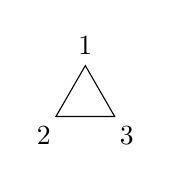
\begin{tikzpicture}[baseline=(a.south)]
   \node[
     draw,
     regular polygon,
     regular polygon sides=3,
     text width=.2em
     ] (a) {};
      \node[above=0pt of a] {$1$};
      \node[below=0pt of a] {$2 \qquad\,\,\, 3$};
 \end{tikzpicture}
\end{figure}
The $+1$ case can be also written as 1, 2 or 3 are in clockwise order. So if you take a triangle and then go clockwise around it from the first element, that the order they are in. The $-1$ are in anticlockwise order. Hence meaning the opposite of clockwise.\\

The six non-zero elements of $\e_{ijk}$:
\begin{align*}
  &\e_{123} = \e_{231} = \e_{312} = +1\\
  &\e_{321} = \e_{213} = \e_{132} = -1 \\
  &\e_{ijk} = 0, \text{ otherwise} \\
\end{align*}

We can take that; $\e_{ijk} = \e_{jki} $ as they are in clockwise order. This also imples $\e_{ijk} = - \e_{jik}$ because if $ijk $ are in clockwise order then $jik$ must be in counterclockwise order.

\subsection{$\e_{i, j, k}$ and cross product}

Let $\vec a = {a}_1 \veci + {a}_2 \vecj + {a}_3 \veck$ and $\vec b = {b}_1 \veci + {b}_2 \vecj + {b}_3 \veck$. Then their cross product is:
$$ \vec a \times \vec b = \left|\begin{matrix}
  \veci & \vecj & \veck \\
  a_1 & a_2 & a_3 \\
  b_1 & b_2 & b_3 \\
\end{matrix}\right| $$

and in suffix notation, we can write the above as; $(\vec a \times \vec b)_i = \e_{ijk} \, a_jb_k $ where $j, k$ are dummy suffixes and must be summed over $1$ to $3$.

\subsection{$\e_{ijk}$ and the scalar triple product}

We can take the scalar triple product, $\vec a \cdot \vec b \times \vec c$, then we can do the following:

\begin{align*}
  \vec a \cdot \vec b \times \vec c &= a_i (\vec b \times \vec c)_i\\
  &= a_i \e_{ijk} b_j c_k \\
  &= \e_{ijk} a_i b_j c_k \\
  &= c_k \e_{ijk} a_i b_j \\
\end{align*}

from the above we show that $\vec a \cdot \vec b \times \vec c = \vec c \cdot \vec a \times \vec b $. We can expand $\e_{ijk}\, a_i\, b_j\, c_k$ to get:
\begin{align*}
  &= \e_{123}a_1b_2c_3 + \e_{231}a_2b_3c_1 + \e_{312}a_3b_1c_2 \\
  &\quad+ \e_{321}a_3b_2c_1 + \e_{213}a_2b_1c_3 + \e_{132}a_1b_3c_2 \\
  &= a_1b_2c_3 + a_2b_3c_1 + a_3b_1c_2 - a_3b_2c_1 - a_2b_1c_3 - a_1b_3c_2
\end{align*}

which is the expanded form of the triple scalar product.

\subsection{A relation between $\e_{ijk}$ and $\kd$}
We are going to prove the following statement:
$$ \e_{ijk}\e_{klm} = \delta_{il}\delta_{jm} - \delta_{im}\delta_{jl} $$
Since all of the coordinate axis are the same, just consider $\displaystyle{i = 1}$:\\

\noindent
If then $\displaystyle{j = 1}$, we get that $\displaystyle{\e_{11k} = 0}$ and so LHS $\displaystyle{= 0}$. Then considering the RHS, we get that $\displaystyle{\delta_{1l}\delta_{1m} - \delta_{1m}\delta_{1l} = 0}$, so equation holds.\\

\noindent
If $\displaystyle{j=2}$, then $\displaystyle{\e_{ijk} = {\e_{12k} = 0}}$, unless $\displaystyle{k=3}$, so then only $\displaystyle{k=3}$ contributes to the sum. So $\displaystyle{\e_{klm} = \e_{3lm}}$, so zero unless $l$ and $m$ are $1$ and $2$. So we can conclude that $\displaystyle{\e_{ijk}\e_{klm} = \e_{123}\e_{312}}$ or $\e_{123}\e_{321}$, so the LHS is either $\pm 1$. Looking at RHS, we have either: $\delta_{11}\delta_{22} - \delta_{12}\delta_{21}$ or $\delta_{12}\delta_{21} - \delta_{11}\delta_{22}$. This gives $\pm 1$ in the same perumtation as the LHS. So equation holds.



\section{Gradient, Divergence and Curl}
\subsection{Gradient}

Assume we have a $f = f(x, y, z)$ or $f = f(x_1,x_2,x_3)$, so a scalar calued function. Then we define grad f as:
$$ \grad = \left(\pd{}{x}\veci + \pd{}{y}\vecj + \pd{}{z}\veck \right)\, f$$
We say grad of $f$ is a differential operator. So:
$$ \grad = \left(\pd{f}{x}\veci + \pd{f}{y}\vecj + \pd{f}{z}\veck \right) $$
and we can write it in suffix notation aswell:
$$ \left[ \grad \right]_i = \pd{}{x_i} \qquad i = 1, 2, 3$$

\subsection{Divergence}

Assume we have a vector field, $\vec{u} = \vec{u} (x, y, z, t)$. We define the divergence of this vector field as;
$$ \nab \cdot \vec{u} = \left(\pd{u_1}{x_1} + \pd{u_2}{x_2} + \pd{u_3}{x_3}\right)$$
Placing this in suffix notation, we get that:
$$ [\nab \cdot \vec{u}]_j = \pd{u_j}{x_j} $$

\subsection{Curl}

the curl of a vector field can be written as:
$$ \nab \times \vec{u} $$
To write this in suffix notation, we can just use the cross produce formula:
$$ [\nab \times \vec{u}]_i = \e_{ijk} \nab_j u_k $$
which then can be manipulated into:
$$ [\nab \times \vec{u}]_i = \e_{ijk} \pd{u_k}{x_j} \qquad j,k = 1, 2, 3 $$
where $i$ is a free index and $j, k$ are dummy suffixes, so $j, k = 1, 2, 3$

\section{Combinations of gradient, divergence and curl}%  $\grad$, $\div(\quad)$ and $\curl(\quad)$}

\subsection{Divergence of Gradient}% $\underline{\nabla} \cdot \underline{\nabla} f$}

If we take $\nab \cdot \grad$ where $f = (x_1, x_2, x_3, t)$. We can write the div of grad as:
\begin{align*}
  \div \grad &= \left(\pd{}{x}\veci + \pd{}{y}\vecj + \pd{}{z}\veck \right) \cdot \left(\pd{f}{x}\veci + \pd{f}{y}\vecj + \pd{f}{z}\veck \right) \\
  &= \pd{}{x_1}\pd{f}{x_1} + \pd{}{x_2}\pd{f}{x_2} + \pd{}{x_3}\pd{f}{x_3}\\
  &= \pd{^2 f}{x_1^2} + \pd{^2 f}{x_2^2} + \pd{^2 f}{x_3^2}\\
  &= \Delta f
\end{align*}

Where the $\Delta = \nab ^2$ is the laplacian. So how do we write this in suffix notation?
\begin{align*}
  \div \grad &= \nab_j[\grad]_j\\
  &= \pd{}{x_j} \pd{f}{x_j}\\
  &= \pd{^2 f}{x_j}\\
\end{align*}

\subsection{Curl of Gradient}

We can write the curl of gradient as:
\begin{align*}
  \left[\curl \grad\right]_i &= \e_{ijk}\nab_j\grad_k\\
  &= \e_{ijk}\pd{}{x_j}\pd{f}{x_k}\\
  &= \e_{ikj}\pd{}{x_k}\pd{f}{x_j}\\
  &= - \e_{ijk}\pd{}{x_k}\pd{f}{x_j}\\
  &= - \e_{ijk}\pd{}{x_j}\pd{f}{x_k} && \text{if $f\in c^2$}\\
  &\implies \curl\grad = 0\\
\end{align*}

\subsection{Gradient of Divergence}
Assume we have a $\vec u$, vector field, and we want $\nab (\div\vec u)$.

\begin{align*}
  [\nab(\div\vec u)]_i &= \nab_i \pd{u_j}{x_j} \\
  &= \pd{}{x_i}\pd{u_j}{x_j} \\
  &= \pd{^2 u_j}{x_i\partial x_j}
\end{align*}

\subsection{Divergence of Curl}
We can write divergence of curl as:
\begin{align*}
  [\div\curl\vec u]_i &= \pd{}{x_i}[\curl\vec u]_i \\
  &= \pd{}{x_i}\e_{ijk}\pd{u_k}{x_j} \\
   \text{$i, j, k = 1, 2, 3$, so $i \leftrightarrow j$}\\
  &= \pd{}{x_j}\e_{jik}\pd{u_k}{x_i} \\
  &= -\e_{ijk}\pd{}{x_j}\pd{u_k}{x_i} \\
  &= -\e_{ijk}\pd{}{x_i}\pd{u_k}{x_j} && \text{as $\vec u \in c^2$} \\
\end{align*}
As $\div(\curl\vec u) = -\div(\curl\vec u)$, then we know that $\div(\curl\vec u) = 0$

\subsection{Curl of Curl}
We can write curl of curl, $ \curl(\curl\vec u)$, as:
\begin{align*}
  [\curl(\curl\vec u)]_i &= \e_{ijk}\pd{}{x_j}(\curl\vec u)_k \\
  &= \e_{ijk}\pd{}{x_j}\e_{klm}\pd{u_m}{x_l} \\
  &= (\delta_{il}\delta_{jm} - \delta_{im}\delta_{jl})\pd{^2 u_m}{x_j\partial x_l} \\
  &= \delta_{il}\delta_{jm}\pd{^2 u_m}{x_j\partial x_l} - \delta_{im}\delta_{jl}\pd{^2 u_m}{x_j\partial x_l} \\
  &= \pd{^2 u_j}{x_j \partial x_i} - \pd{^2 u_i}{x_j \partial x_j}\\
  &= \pd{}{x_i}\pd{u_j}{x_j} - \pd{^2 u_i}{x_j^2} \\
  &= [\nab(\div\vec u)]_i - [\Delta\vec u]_i\\
  &= [\nab(\div\vec u) - \nab^2\vec u]_i\\
\end{align*}

\section{Scalar Field / Vector Fields Defintions}

A scalar or vector quantity is said to be a {\color{blue} field }if it is a function of position. Examples
\begin{enumerate}
  \item {\color{orange}Temperature} is a scalar field, $T = T(x, y, z) = T(\vec r)$
  \item {\color{orange}Pressure and Density} are also scalr fields $P = P(\vec r)$ and $\rho = \rho(\vec r)$
  \item if a physical quantity is a scalar we speak of a scalar field or function of position.
\end{enumerate}

\noindent
If a physical quantity is a vector, such as force $\vec F = \vec F(x, y, z)$. We speak of a {\color{blue}vector field} or {\color{blue}vector function}. \\

\noindent
A {\color{blue} vector-valued function }is an $f: A\subset \R^n \mapsto \R^m$. So, for each $\vec x = (x_1,\,\dots\,, x_n) \in A$, $f$ assigns a value $f(\vec x)$, an m-tuple, in $\R^m$. These functions, $f$, are called vector-valued functions if $m>1$ and scalar if $m=1$.\\

\noindent\fbox{\parbox{0.475\textwidth}{\begin{example}{
  Take the function, $f: (x, y, z) \mapsto (x^2 + y^2 + z^2)^\frac{3}{2}$
}\end{example}\begin{solution}{
  It's a scalar function from $\R^3$ to $\R$.
}\end{solution}}}\vspace{10pt}

\noindent\fbox{\parbox{0.475\textwidth}{\begin{example}{
   Take the function $g: (x_1, x_2, x_3) \mapsto (x_1x_2x_3, \sqrt{x_1x_3}) $
}\end{example}\begin{solution}{
  This is a vector valued function from $\R^3$ to $\R^2$
}\end{solution}}}\vspace{10pt}

To specify a temperature $T$ in a region $A$ of space requires a function $T$, $T: A\subset \R^m \mapsto \R$. $T = T(x, y, z)$.\\

\noindent
To specify the velocity of a fluid moving in space requires a map, $\vec v: \R^4 \mapsto \R^3$ where $\vec v (x, y, z, t)$ is the velocity of the fluid at $(x, y, z)$ at time $t$.\\

\noindent
When $f: U\subset\R^n \mapsto \R$, we say that $f$ is a real valued function of $n$-variables with domain $U$.\\

\noindent
Let $f: U:\R^n \mapsto \R$, then graph $f = \{ (x_1, x_2,\, \dots\,, x_n) \in \R^{n + 1} : (x_1,\, \dots\,, x^n)\}$
If $n= 1$, then we can conclude that graph $f$ is curve in $\R^2$ and if $n=2$, then graph $f$ is a surface in $\R^3$.

\subsection{Level Sets, Curves and Surfaces}
A level set is a subset of $\R^3$ on which $f$ is constant. For example, for $f(x, y, z) = x^2 + y^2 + z^2$, the set where $x^2 + y^2 + z^2 = 1$ is alevel set. A level set is a set of $(x, y, z): f(x, y, z) = c$ where $c \in \R$.\\

For functions $f(x, y)$, we speak of level curves or contours. example, $f: \R^2 \mapsto \R$, $f(x, y) = x + y + 2$, has as it's graph the inclined plane $z = x + y + 2$. The plane intersects the $xy$ plan where $z = 0$ in the line $y = -x - 2$ and the $z$-axis at $(0, 0, 2)$. For any $c \in \R$, the level curve of $c$ is the straight line: $y = -x + (c-2): L_c \{(x, y): y = - x + c - 2 \}\subset \R^2$













\end{document}
